\chapter{\'Etat de l'art}
Nous avons recherché plusieurs projet proche de la desserte robotisée.

\section{Robot Numéro 1 de Firstclass Robotics}
Ce projet est très proche de notre desserte d'un point de vue fonctionnel. En effet, il est prévu pour servir lors de reception. il est déjà en service et peut être loué au près de First Class Robotique. 

\begin{figure}[h]
\begin{center}
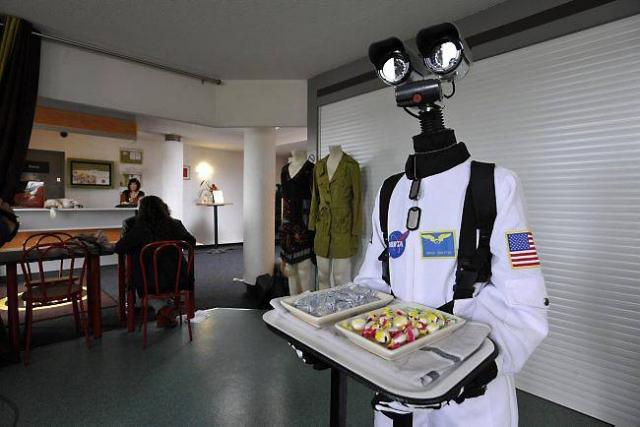
\includegraphics[scale=0.55]{Images/robot_n1.jpg}
\caption{robot Numéro 1}
\label{robot Numéro 1}
\end{center}
\end{figure} 

Ce robot à été conçu par Bernard MARTI, qui à notamment été professeur
de robotique à l'INSA de Lyon. Ce robot à clairement été conçu d'un
point de vue industriel et dans une optique de faire un robot à bas
coût. Il coute 15000 euros.

\subsection{caractéristique}
le robot fait 1m55, à une autonomie de 12h, et utilise un système de
vision basé à la fois sur des capteur infrarouge et et des capteurs
ultrasons et permettant une vision à 12m.

Le robot ce caractèrise aussi par une absence de communication avec
une base, permettant de le rendre insensible à tout pratage
informatique. il est complètement autonome et ne necessite pas de
cartographie. Bernard MARTI parle d'ailleur de programmation
insectoïde et réduite au minimum.

A noté qu'une version "plus" existe également, plus axée assistance.

\subsection{contexte}

Une différence majeure de ce robot par rapport à notre projet est que ce robot n'essaye pas d'imiter un serveur, mais se presente plutôt comme un robot d'aide au serveur. Le concepteur du robot indique par ailleurs que le robot à été plutôt bien accueilli par les professionel qui officiait a ses côtés. 

\section{Care O Bot}

Le care O bot s'écarte un peu de notre projet mais reste à étudier. Il
s'agit d'un robot d'aide à la personne, équipé d'un bras articulé et
d'un plateau. il est construit par Fraunhofer, une entreprise
allemande.

\subsection{caractéristique}

\begin{figure}[h]
\begin{center}
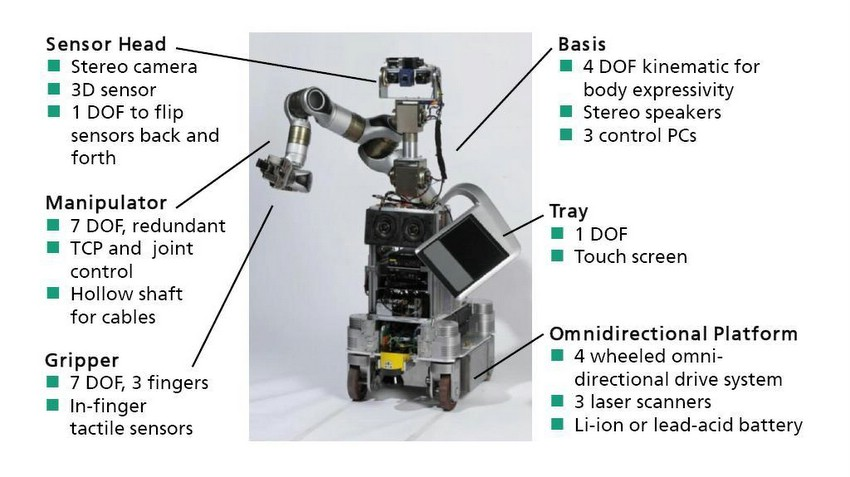
\includegraphics[scale=0.55]{Images/cob3-hardware.jpg}
\caption{caractéristique du careObot3}
\label{caractéristique du careObot3}
\end{center}
\end{figure}

Le robot roule d'une manière lente et fluide. Il utilise des caméras et des capteur de profondeurs pour se reperer, ainsi qu'un système de cartographie. Son bras possède 7 degré de liberté. pour intéragir, il dispose d'une tablette tactile sur son plateau ainsi que d'une reconnaissance faciale et auditive. Il dispose aussi d'haut parleur pour communiquer.

\subsection{contexte}

Ce robot évolue dans un contexte très différents de notre desserte. Il se trouve chez des particuliers ou dans des maisons de retraites. Il n'a donc pas les mêmes contraintes en terme de gestion de foule et de déplacement. En revanche il peut-être très interessant d'étudier sa façon de servir et de s'approcher des humains.

\newpage

\section{Dalu Robot}

Dalu Robot n'est pas un robot, mais un restaurant chinois qui utilise plusieurs robot pour servir leurs clients. Ces robot sont assez rudimentaires en soi, puisqu'ils suivent une ligne blanche au sol qui fait le tour de la pièce et s'arretes losrqu'un humain s'arrête.

\begin{figure}[h]
\begin{center}
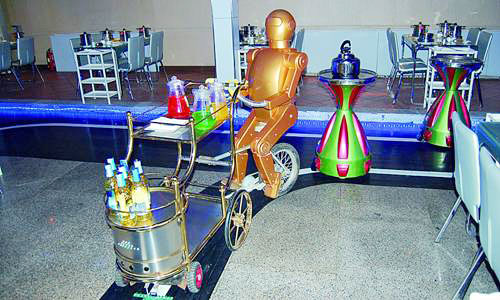
\includegraphics[scale=0.55]{Images/dalu-robot-1.jpg}
\caption{exemple de robot chez Dalu Robot}
\label{exemple de robot chez Dalu Robot}
\end{center}
\end{figure}


